\chapter{Introduction: Plasmas and Tokamak Plasmas}
    Nuclear fusion energy has the potential to provide a nearly unlimited source of clean and safe energy. Fusion reactions do not produce harmful greenhouse gases or long-lived radioactive waste and provide no risk of meltdown, making it a sustainable solution to meet the world's growing demand for energy, from a stable and renewable source: hydrogen (and its isotopes). With the world's energy demands continuously growing, fusion energy presents an attractive option for meeting these demands in a safe and sustainable manner.

    \shortline
      
    Tokamaks---devices that use strong magnetic fields to contain and control plasmas at exceedingly high temperatures in order to achieve fusion---have proven over the past decades to be an effective leading option for producing and sustaining fusion. Unlike other similar devices, such as stellarators or Z-pinch devices, tokamaks have a relatively simple and well-studied  design with comparatively straightforward engineering, making them easier to scale up to commercial-scale reactors. With its first plasma scheduled for late 2025 \cite{ITER_schedule}, the International Thermonuclear Experimental Reactor (ITER) will be the world's largest tokamak \cite{Meade_2009, ITER_plan}, building towards DEMO: a proposed class of demonstration tokamak, with a target for commercial operation in the 2050s.

    Because of these factors, tokamaks have received extensive funding and support from governments and private organizations around the world, making them potentially the most widely researched and developed fusion technology.

    These factors combined make tokamaks one of the world's best solutions for fusion energy, and arguably the most likely to achieve practical and commercial fusion reactor in the coming decades.

    \begin{figure}[!ht]
        \centering
        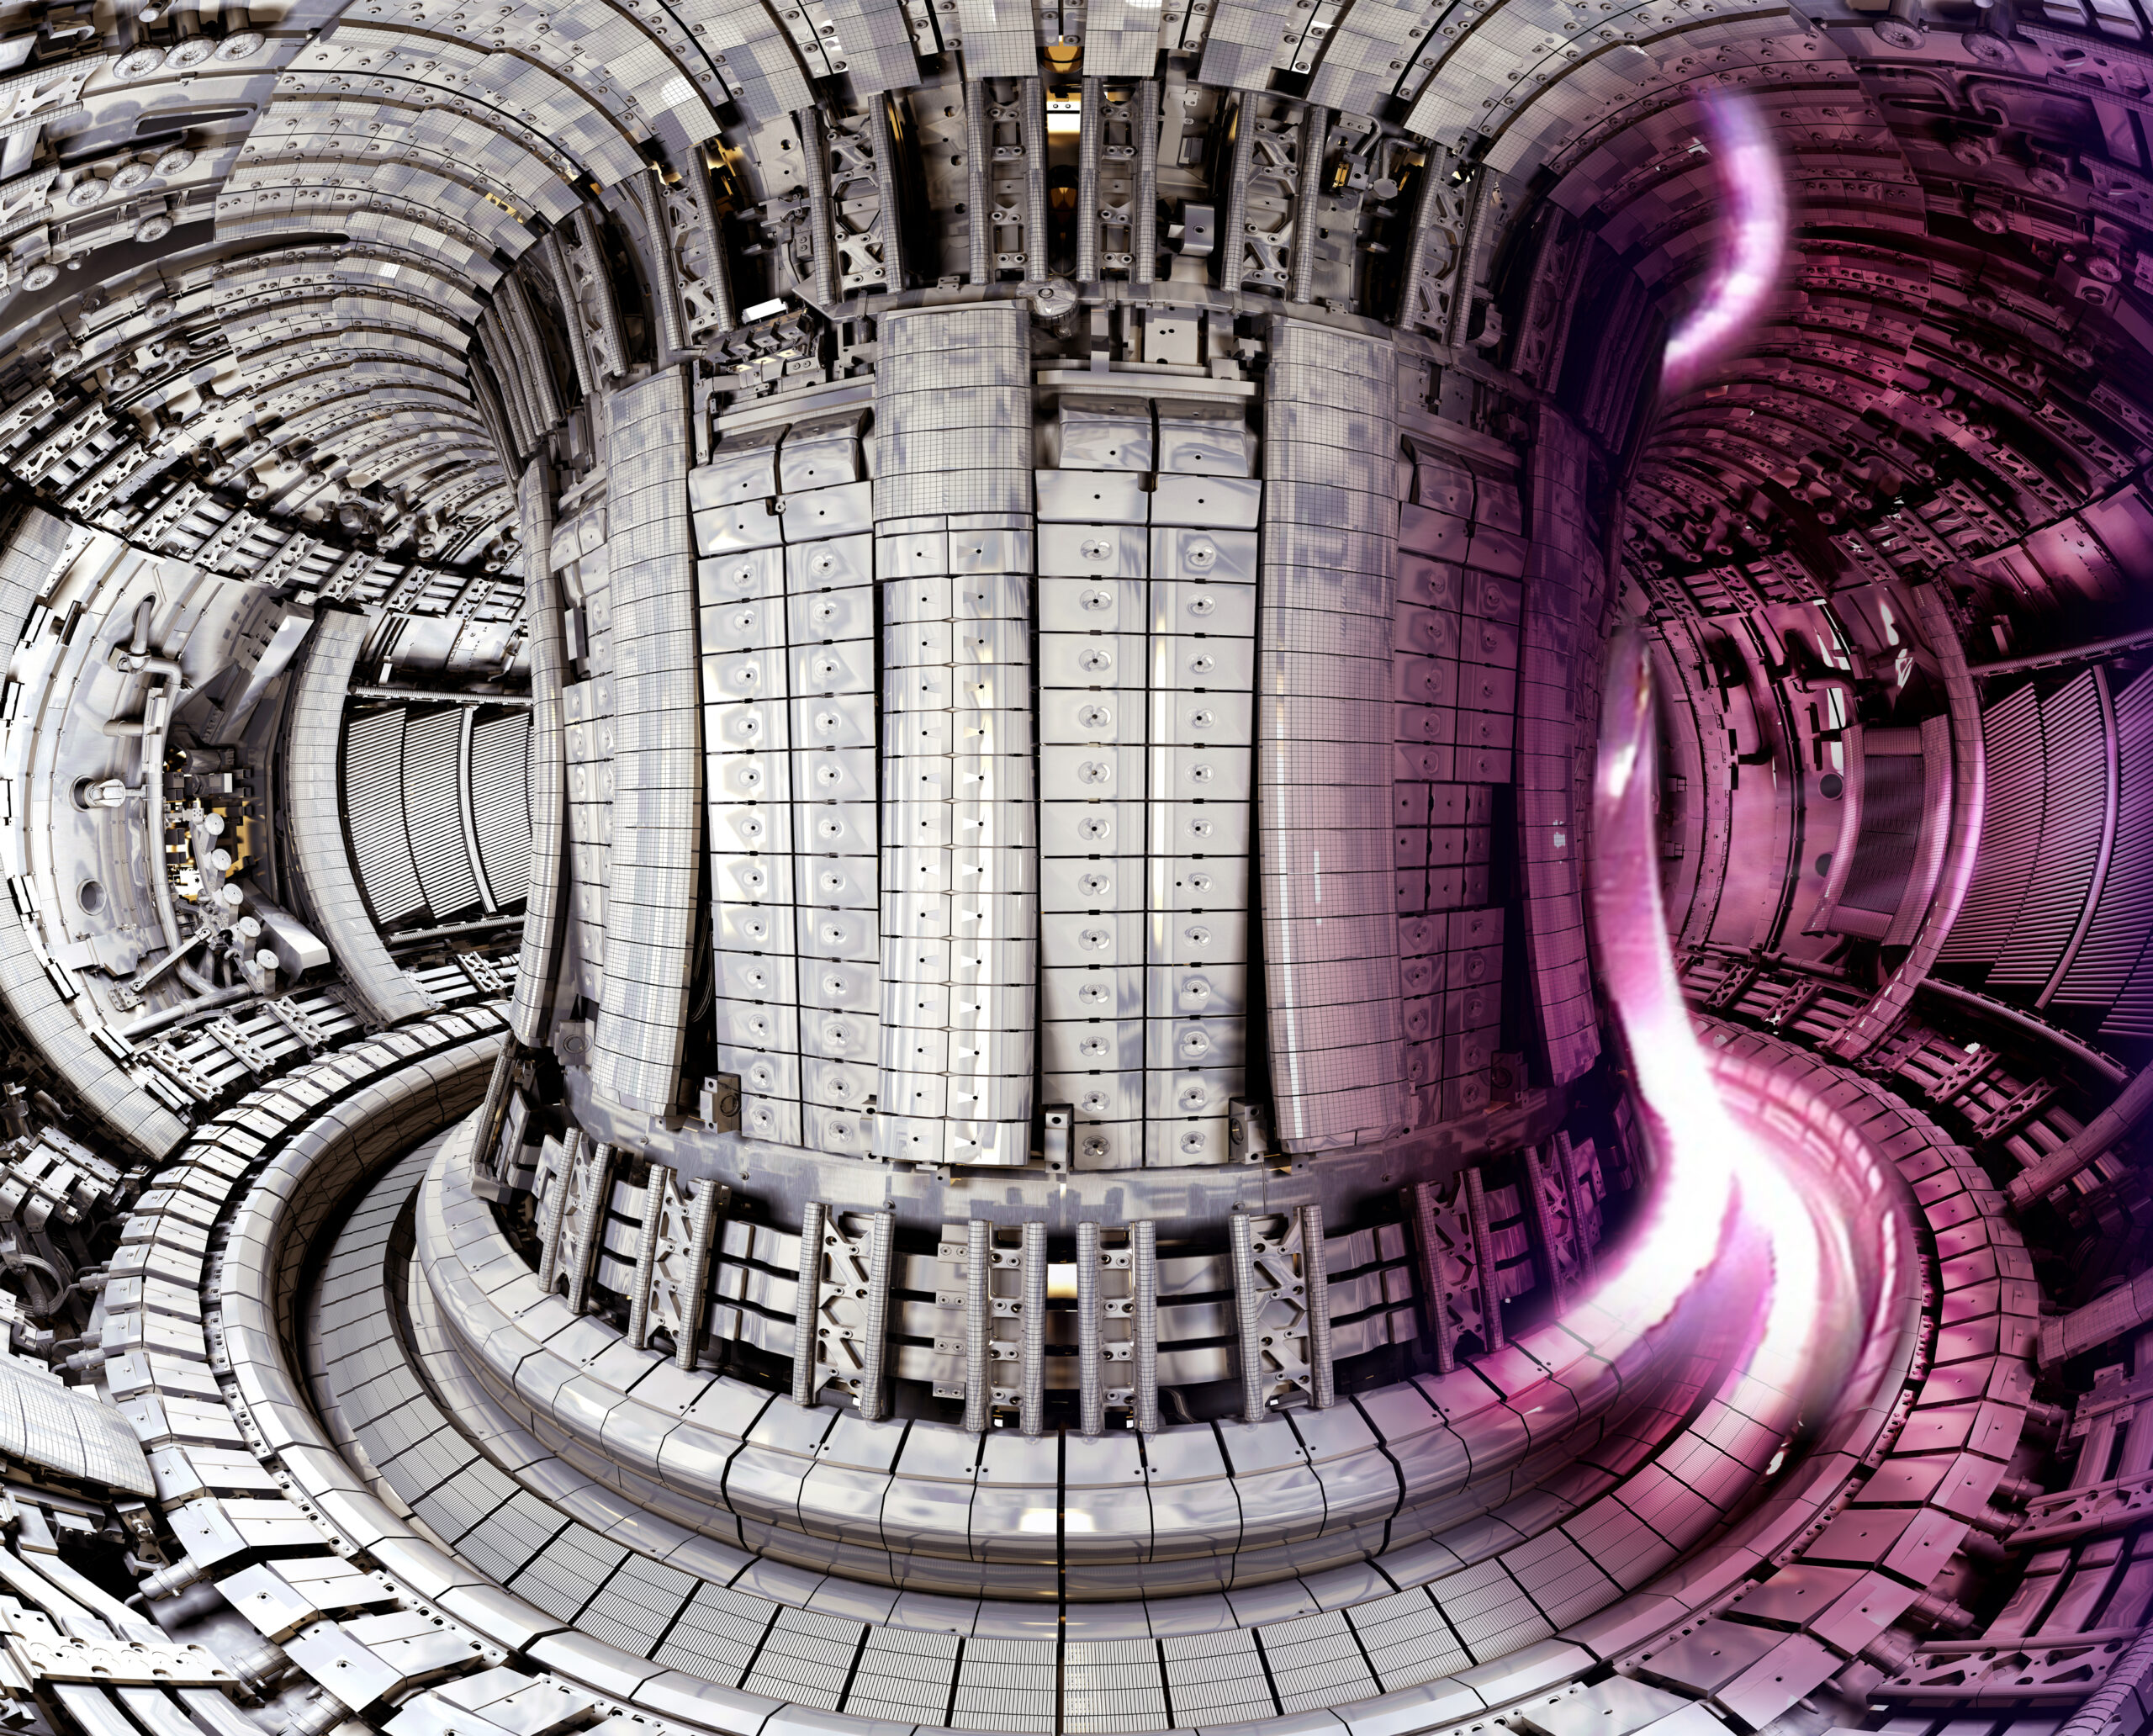
\includegraphics[width = 0.8\textwidth]{0 - introduction/images/JET.jpg}
        \caption{Illustration of the interior of the Joint European Torus (JET) reactor, located at the Culham Centre for Fusion Energy (CCFE). At the time of creation, JET was the largest tokamak in the world. (Source: CCFE)}
    \end{figure}

    \shortline

    The physical and numerical modeling of plasmas is a crucial area of study for tokamaks because it helps to understand and predict the behavior of the hot plasma in the containment vessel. The plasma must be maintained at high temperatures and densities in order to achieve fusion, and understanding its behavior is essential for optimizing the conditions in the tokamak and improving the fusion efficiency. Plasma modeling allows the simulation of various scenarios, such as changes in the magnetic fields or the heating methods used, and the observation of how these affects the plasma, allowing researchers and engineers to make informed decisions about how to increase the energy yield.

    In addition, plasma modeling helps to identify and resolve potential problems that may arise during the fusion reaction, such as instabilities in the plasma or unwanted interactions with the chamber walls. By using computer simulations, these issues can be identified and resolved before they occur outside of the simulation, making the process safer and more efficient.
    
    \shortline

    \begin{remark}
        For a detailed introduction to plasmas and their modeling, and the great difficulties these pose in tokamak-like environments, see \cite{addendum_I}. I have chosen to omit this in this document for brevity.
    \end{remark}
